\chapter{Considerazioni finali e proposte per lavori futuri}
\label{ch:conclusionilavorifuturi}

In questo capitolo andremo a riportare alcune considerazioni circa i metodi discussi per il ranking delle tratte ferroviarie e delle stazioni che su di esse insistono al fine di proporre spunti per i lavori futuri. Inoltre verranno evidenziate alcune inesattezze riscontrate nei dataset utilizzati.
\newline
In conclusione è presente un riepilogo del lavoro svolto.
\section{Proposte per lavori futuri sul metodo di ranking delle stazioni ferroviarie}
Benchè il metodo di ranking delle stazioni ferroviarie di cui abbiamo discusso nella sezione \ref{metodoNuovo} abbia consentito il raggiungimento dell'obiettivo preposto per tale laboratorio (esposto nel Cap. \ref{ch:introduzione}) è opportuno comunque fare alcune considerazioni a riguardo, al fine di ottenere degli spunti per eventuali lavori futuri. Come abbiamo già discusso nella sezione \ref{discussioneRisultati}, il metodo NMC ha buone performance e riesce generalmente ad individuare quali sono le stazioni ferroviarie che necessitano di un monitoraggio più frequente da parte degli organi competenti data la loro esposizione al rischio di frane ma presenta alcune limitazioni che ci hanno consentito di realizzare alcune considerazioni a partire dalle quali abbiamo ipotizzato alcuni spunti operativi per lavori futuri. Uno tra questi consiste nell'idea di poter considerare nell'intorno del punto \textit{$b_i$} che individua l'edificio della stazione ferroviaria un triangolo in cui \textit{$b_i$} rappresenta il baricentro (vedi Fig. \ref{baricentro}).
\begin{figure}[hpt]
	\centering
	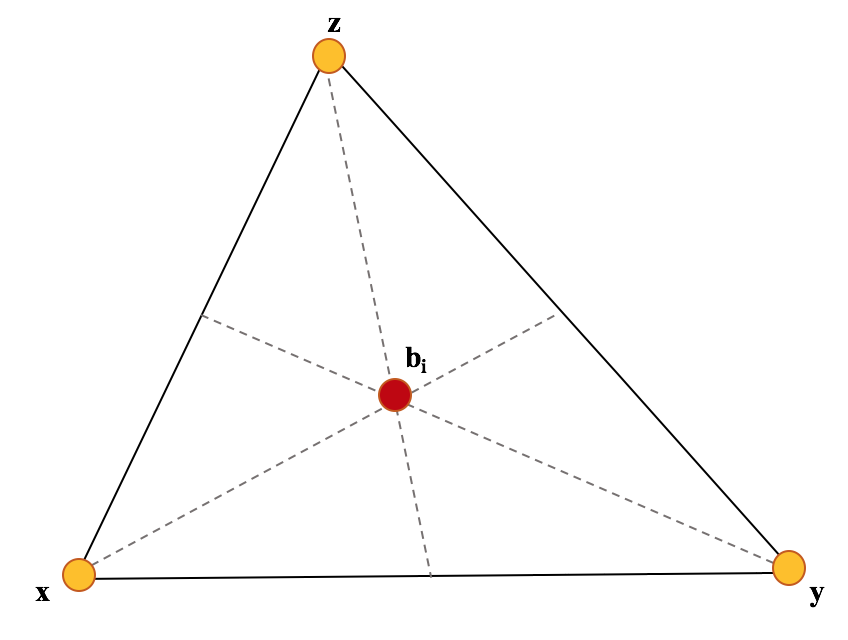
\includegraphics[width=0.5\linewidth]{img/baricentro}
	\caption{Triangolo costruito nell'intorno di \textit{$b_i$}}
	\label{baricentro}
\end{figure}

Sui vertici di tale figura sarà possibile calcolare il valore di \textit{exposure} corrispondente così come esposto nella Sez. \ref{metodoNuovo}: Il valore di \textit{exposure} associato alla stazione ferroviaria \textit{$b_i$} sarà pari alla loro media aritmetica.
Così facendo, considerando più punti nell'intorno dell'edificio sarà possibile ottenere valori di \textit{exposure} più coerenti con la reale conformazione morfologica del terreno circostante, superando di conseguenza le limitazioni di cui abbiamo discusso nella Sez. \ref{discussioneRisultati}.
 
\section{Proposte per lavori futuri sul metodo di ranking delle tratte ferroviarie}
Il metodo NMCE, discusso nella Sez. \ref{metodoLinee}, proposto per il ranking delle tratte ferroviarie circa il loro livello di esposizione al rischio di frane ci ha consentito di realizzare una valutazione circa le loro potenziali pericolosità. Uno spunto per dei lavori futuri al fine di migliorare l'affidabilità dei risultati ottenuti potrebbe essere quello di introdurre dei dataset circa le gallerie e i ponti ferroviari dislocati lungo la rete ferroviaria. Questi infatti sono nel nostro metodo NMCE fonte di falsi positivi nella classificazione in fasce di rischio dei segmenti della rete ferroviaria, come abbiamo già discusso nella Sez. \ref{discussioneLinee}.
\section{Considerazioni sui dataset}
Nella valutazione delle performance dei metodi proposti non è possibile prescindere dalla consapevolezza che i dataset utilizzati potrebbero essere incompleti o potrebbero presentare imprecisioni. 
Uno spunto per dei lavori futuri potrebbe essere quello di utilizzare un dataset della rete ferroviaria e delle stazioni che insistono su di essa aggiornato, tale da limitare le inesattezze dei risultati. Infatti, in seguito ad accurate ricerche effettuate in rete, risulta evidente che alcune tratte, nonchè alcune stazioni situate lungo di esse, sono inattive o in fase di smantellamento. I portali che abbiamo utilizzato maggiormente sono quello proposto da Trenitalia (\url{http://www.rfi.it/rfi/LINEE-STAZIONI-TERRITORIO/Nelle-regioni/Abruzzo/La-rete-oggi-in:-Abruzzo}) e \url{http://www.ferrovieabbandonate.it/}.
\newpage
Qui di seguito alcune foto di stazioni ferroviarie ormai dismesse o in disuso: Archi (Fig. \ref{archi}) , Perano (Fig. \ref{perano}), Pettorano sul Gizio (Fig. \ref{pettorano}) e Civitaluparella (Fig. \ref{civitaluparella}).
\begin{figure}[h]
\centering
\begin{minipage}[c]{.40\textwidth}
\centering\setlength{\captionmargin}{0pt}%
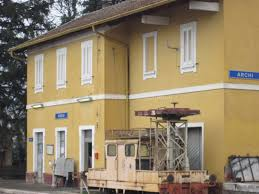
\includegraphics[width=.60\textwidth]{img/archi}
\caption{Stazione di Archi}
\label{archi}
\end{minipage}%
\hspace{10mm}%
\begin{minipage}[c]{.40\textwidth}
\centering\setlength{\captionmargin}{0pt}%
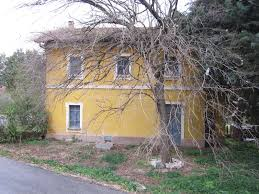
\includegraphics[width=.60\textwidth]{img/perano}
\caption{Stazione di Perano}
\label{perano}
\end{minipage}
\begin{minipage}[c]{.40\textwidth}
\centering\setlength{\captionmargin}{0pt}%
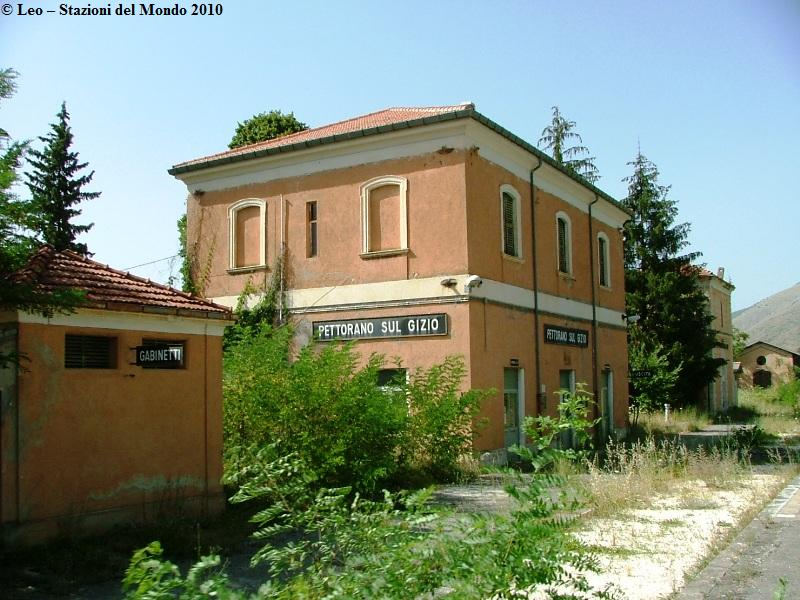
\includegraphics[width=.60\textwidth]{img/pettorano}
\caption{Stazione di Pettorano}
\label{pettorano}
\end{minipage}%
\hspace{10mm}%
\begin{minipage}[c]{.40\textwidth}
\centering\setlength{\captionmargin}{0pt}%
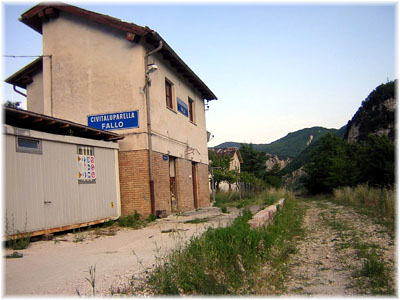
\includegraphics[width=.60\textwidth]{img/civitaluparella}
\caption{Stazione di Civitaluparella}
\label{civitaluparella}
\end{minipage}
\end{figure}

E' necessaria inoltre un'altra riflessione circa i dataset utilizzati, quella circa il dataset delle zone in cui è stato deframmentato il territorio abruzzese. Il dataset in nostro possesso è l'output di un metodo che sfrutta un algoritmo che si basa sul \textit{Diagramma di Voronoi} per decomporre il territorio, per cui le zone ottenute potrebbero non rispecchiare in maniera coerente le caratteristiche morfologiche del terreno. Bisogna inoltre considerare che il valore numerico che quantifica la pericolosità di frana di ogni zona è strettamente legato alle curve di livello che sono presenti in tale zona e non tiene conto di quelle che sono le caratteristiche litologiche del terreno. 
Uno spunto per i lavori futuri potrebbe essere quello di utilizzare un dataset delle zone che presenti maggiore affidabilità circa la morfologia e le caratteristiche del territorio.
\section{Considerazioni finali}

L’obiettivo di questo studio è stato fornire una classifica circa le stazioni e le linee ferroviarie in base al loro livello di esposizione al rischio frane. Sono stati proposti rispettivamente due metodi al fine di raggiungere tale scopo.  Successivamente è stata progettata una base di dati spaziale atta a contenere i dataset presi in input. Nel nostro caso di studio questi ultimi hanno interessato la regione Abruzzo. La base di dati spaziale è stata implementata tramite il DBMS PostgreSQL servendoci dell’estensione spaziale PostGIS. Sono state implementate delle UDF, e definite apposite query, tramite le quali poter raggiungere l’obiettivo preposto. Dopo un’analisi dei risultati ottenuti, si è proceduto alla discussione circa le criticità dei metodi e dei dataset in input. E' opportuno sottolineare come i metodi proposti non abbiano la pretesa di restituire valori assoluti circa l’esposizione al pericolo di frane, bensì quello di fornire una metodologia valida applicabile e ovviamente migliorabile per determinare delle classifiche grazie alle quali è possibile individuare le stazioni e le tratte ferroviarie che sono maggiormente esposte al pericolo di smottamenti. I risultati finali sono migliorabili sulla base degli spunti offerti durante la trattazione.  